% TODO : TP : exemples des films, version python
% exemples de requêtes
% puis version SQL.

\section{Introduction}

On s'intéresse au problème de la gestion d'un gros volumes de données, ainsi qu'à celui de la recherche sur ces données.
%\clearslide{}
\subsection{Exemple : IMDB}

C'est une base de données sur les films, les réalisateurs et les acteurs, qui est accessible en ligne (\url{http://www.imdb.com/stats}).
Elle a environ $6\times 10^{7}$ visiteurs par mois (\url{http://fr.wikipedia.org/wiki/IMDB}).

Quelques données chiffrées : cette base de donnée répertorie
\begin{itemize}
\item $\approx 4,7\times 10^{6}$ titres ;
\item $\approx 8,7\times 10^{6}$ personnes (dont $\approx 3,3\times 10^{6}$ acteurs et actrices).
\end{itemize}
(source : \url{http://www.imdb.com/stats}, le 16 février 2018)

Au regard des standards actuels IMDB est
\begin{itemize}
\item une base de données de taille moyenne ;
\item avec un nombre de consultations moyen.
\end{itemize}

%\clearslide{}

\subsection{Et si on faisait notre IMDB?}

C'est un peu ambitieux, on va simplifier un peu.

On commence par se poser les questions suivantes. 
\begin{itemize}
\item Comment modéliser ce problème ?
\item Comment représenter les données à stocker ?
 % ??\item \xout{Comment faire une interface web ?}
\end{itemize}

\section{Modèle conceptuel des données}

On a besoin de modéliser le problème qu'on aborde \textbf{avant} de commencer à programmer.
C'est une tâche très difficile. On peut retenir deux points fondamentaux. 
\begin{itemize}
\item Cela nécessite une collaboration entre des spécialistes du domaine et des informaticiens\footnote{En
    général, cela demande une collaboration entre informaticiens de
    spécialités différentes.}.
\item En cas d'hésitation ou d'ambiguïté, les informaticiens doivent \textbf{refuser} de choisir.
\end{itemize}

%\clearslide{}
\subsection{Le modèle entité-association}
De l'anglais \textbf{Entity-Relationship model}. 

C'est :
\begin{itemize}
\item une façon de  modéliser les  données à traiter ;
\item un modèle \textbf{conceptuel} de  données (MCD).
\end{itemize}
Le mot \textbf{conceptuel} doit s'entendre par opposition à  l'\textbf{implantation} concrète de la base de données (qui donne le modèle \textbf{physique} de données, MPD).

On l'appelle ainsi car il distingue :
\begin{itemize}
\item les entités (objets d'intérêt) ;
\item des associations (liens) entre ces entités.
\end{itemize}
%\clearslide{}
\subsection{Entités}
Ici, dans notre exemple de base de donnée cinématographique, nous choisissons comme entités :
  \begin{enumerate}
  \item les films ;
  \item les personnes (acteurs, réalisateurs, scénaristes, etc.).
  \end{enumerate}

\begin{rem}
  On pourrait rajouter : les entreprises (producteurs), les livres
  (dont sont tirés certains scénarios), les pays (où ont eu lieu le
  tournage, du producteur, où sont distribués les films), les langues
  (des films), les versions d'un même film (langues, montages), \textbf{etc}.
\end{rem}


%\clearslide{}
Pour chaque entité, on considère les données suivantes. 
\begin{description}
\item[Pour les films] Titre, date de sortie ;
\item[Pour les personnes] Nom, prénom, date de naissance.
\end{description}
\begin{rem}
  Là encore, c'est un choix, on aurait pu allonger cette liste. 
\end{rem}

%\clearslide{}
\subsection{Associations}
Ici, on ne considère dans notre exemple que deux types de relation :
  \begin{enumerate}
  \item «joue dans» (Clint Eastwood joue Blondin dans \textbf{Le bon, la brute
      et le truand} et Walt Kowalski dans \textbf{Gran Torino}) ;
  \item «a réalisé» (Clint Eastwood a réalisé \textbf{Invictus} et
    \textbf{Gran Torino}).
  \end{enumerate}

%\clearslide{}

Quelques informations pertinentes sont à prendre en compte sur ces relations.
\begin{itemize}
\item Tout film a été réalisé par une personne.
\item Tout film a été réalisé par au plus une personne (ce n'est pas forcément vrai pour tout film !).
\item Toute personne peut avoir réalisé $0$, $1$ ou plusieurs films.
\item Toute personne peut avoir joué dans $0$, $1$ ou plusieurs films.
\item Tout film a $0$, $1$ ou plusieurs acteurs.
\item Lorsqu'une personne joue dans un film, il est intéressant de
  savoir quel est son rôle (elle peut alors jouer un ou plusieurs rôles).
\end{itemize}
Clairement, nous sommes ici dans une étape de modélisation, qui possède donc des limites.

On remarquera que nous pourrions avoir intérêt à introduire une entité supplémentaire : les personnages. Pour chaque personnage, on ne considèrera que son nom. 
%\clearslide{}

\subsection{Diagramme entité/association}

On représente la modélisation précédente du lien entre les entités et les associations de notre projet de base de données cinématographique par le diagramme suivant.
\begin{center}
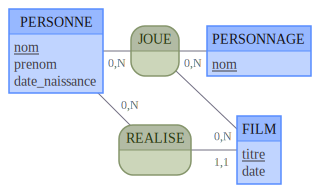
\includegraphics[height=5cm]{films.png}
\end{center}
%\clearslide{}

On porte sur le diagramme des indications pour préciser comment
fonctionnent les relations.

Considérons la relation $R$ des $(p,f)$ où :
\begin{itemize}
\item $p$ est une personne ;
\item $f$ est un film ;
\item $p$ a réalisé $f$.
\end{itemize}
\begin{rem}
  La relation $R$ modélise mathématiquement l'association «REALISE»
\end{rem}

%\clearslide{}

Dans $R$, par notre modélisation, on a les propriétés suivantes. 
\begin{itemize}
\item Un même film apparaît au moins une fois et au plus une fois
  (tout film a un unique réalisateur), d'où le «$1,1$» sur le trait
  reliant «REALISE» à «FILM» sur le diagramme.
\item Une même personne peut apparaître $0$, $1$ ou plusieurs fois,
  d'où le «$0, N$» sur le trait reliant «REALISE» à «PERSONNE».
\end{itemize}

On utilise le même principe pour renseigner le diagramme de la relation «JOUE».

%\clearslide{}
\section{Modèle logique des données}
\subsection{Tables}
On représente ces entités et ces associations par des tables. 
%\clearslide{}

Par exemple, voici une table pour les personnes.
\begin{center}
\begin{tabular}{lll}
\toprule
nom & prénom & date\_naissance\\
\midrule
Kubrick&Stanley&1928\\
Spielberg & Steven& 1946\\
Eastwood & Clint& 1930\\
Cumberbatch & Benedict & 1976\\
Freeman & Martin& 1971\\
Leone & Sergio & 1929 \\
McGuigan & Paul & 1963\\
Sellers&Peter&1925\\
\bottomrule
\end{tabular}
\end{center}
%\clearslide{}
Une pour les films.
\begin{center}
\begin{tabular}{ll}
\toprule
  titre & date\\
\midrule
  Gran Torino & 2008\\
  The good, the Bad and the Ugly& 1966\\
  Study in Pink & 2010\\
  Schindler's List& 1993\\
  Dr Strangelove&1964\\
  Invictus& 2009\\
\bottomrule
\end{tabular}
\end{center}
%\clearslide{}
Une pour les personnages.
\begin{center}
\begin{tabular}{l}
\toprule
  nom\\
\midrule
  Walt Kowalski\\
  Blondie\\
  Shelock Holmes\\
  Dr John Watson\\
  Dr Strangelove\\
  Group Capt. Lionel Mandrake\\
  President Merkin Muffley\\
\bottomrule
\end{tabular}
\end{center}
%\clearslide{}
Une pour l'association «JOUE».
\begin{center}
  \begin{tabular}{llll}
    \toprule
    nom & prenom & titre & nom (de personnage)\\
    \midrule
    Eastwood & Clint & {\small The good, the Bad and the Ugly}& Blondie\\
    Eastwood & Clint & Gran Torino& Walt Kowalski\\
    Cumberbatch&Benedict&Study in Pink& Sherlock Holmes\\
    Freeman & Martin&Study in Pink&Dr John Watson\\
    Selers & Peters&Dr Strangelove&Dr Strangelove\\
    Selers & Peters&Dr Strangelove&{\small Group Capt. Lionel Mandrake}\\
    Selers & Peters&Dr Strangelove&{\small President Merkin Muffley}\\
\bottomrule
  \end{tabular}
\end{center}
%\clearslide{}
Une pour l'association «REALISE».
\begin{center}
\begin{tabular}{lll}
\toprule
  titre & nom (réalisateur)&prénom (réalisateur)\\
\midrule
  Gran Torino & Eastwood&Clint\\
  { The good, the Bad and the Ugly}&Leone&Sergio\\
  Study in Pink &  McGuigan & Paul\\
  Schindler's List& Spielberg&Steven\\
  Dr Strangelove& Kubrick&Stanley\\
  Invictus & Eastwood&Clint\\
\bottomrule
\end{tabular}
\end{center}
%\clearslide{}

\subsection{Vers une implantation?}

On peut considérer ces tables comme des ensembles de $n$-uplets ($n=3$
pour la table «PERSONNE», $n=2$ pour «FILMS», $n=4$ pour «JOUE», $n=3$
pour «REALISE»).

Ces ensembles de $n$-uplets peuvent être implantés en python par des
listes de listes:

\begin{lstlisting}
FILMS = [
 [ 'Gran Torino', 2008 ],
 [ 'The good ...', 1966 ],
 ...
]
...
\end{lstlisting}

Ce modèle à  base de tables, appelé \textbf{modèle  logique des données}
est plus proche  de l'implantation que le modèle  conceptuel. Il reste
cependant à  faire quelques choix  avant de pouvoir vraiment  passer à
une implantation.

\subsection{Une erreur de conception}

Dans la table «JOUE», on a décidé de ne mettre que le nom et le prénom
de l'acteur car on considère que cela suffit à représenter l'acteur.

C'est en général une très très mauvaise idée: que se passe t-il si
deux personnes ont le même nom et prénom?

Une solution classique (en gestion) : attribuer un numéro unique (de
dossier, de personne, \ldots{}), \textbf{l'identifiant}.

On modifie alors le diagramme entité/association comme suit. 
\begin{center}
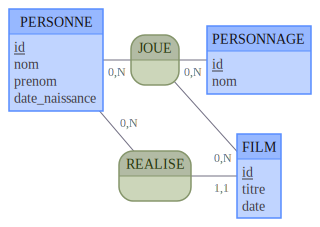
\includegraphics[height=5cm]{films-id.png}
\end{center}
%\clearslide{}

Les tables d'entités sont alors modifiées comme suit.
\begin{center}
\begin{tabular}{llll}
\toprule
id & nom & prénom & date\_naissance\\
\midrule
1&Kubrick&Stanley&1928\\
2&Spielberg & Steven& 1946\\
3&Eastwood & Clint& 1930\\
4&Cumberbatch & Benedict & 1976\\
5&Freeman & Martin& 1971\\
6&Leone & Sergio & 1929 \\
7&McGuigan & Paul & 1963\\
8& Sellers&Peter&1925\\
\bottomrule
\end{tabular}
\end{center}
%\clearslide{}

\begin{center}
\begin{tabular}{lll}
\toprule
id & titre & date\\
\midrule
1 & Gran Torino & 2008\\
2 & The good, the Bad and the Ugly& 1966\\
3 & Study in Pink & 2010\\
4 & Schindler's List& 1993\\
5 & Dr Strangelove&1964\\
6 & Invictus & 2009\\
\bottomrule
\end{tabular}
\end{center}
%\clearslide{}

\begin{center}
\begin{tabular}{ll}
\toprule
id & nom\\
\midrule
1 & Walt Kowalski\\
2 & Blondie\\
3 & Shelock Holmes\\
4 & Dr John Watson\\
5 & Dr Strangelove\\
6 & Group Capt. Lionel Mandrake\\
7 & President Merkin Muffley\\
\bottomrule
\end{tabular}
\end{center}
%\clearslide{}

L'association «JOUE» est donc modifiée de cette manière.
\begin{center}
  \begin{tabular}{lll}
    \toprule
    idacteur & idfilm & idpersonnage\\
    \midrule
    3 & 2 & 2\\
    3 & 1 & 1\\
    4 & 3 & 3\\
    5 & 3 & 4\\
    8 & 5 & 5\\
    8 & 5 & 6\\
    8 & 5 & 7\\
\bottomrule
  \end{tabular}
\end{center}
%\clearslide{}
Et voici celle pour l'association «REALISE».
\begin{center}
\begin{tabular}{ll}
\toprule
  idfilm & idrealisateur\\
\midrule
  1 & 3\\
  2 & 6\\
  3 & 7\\
  4 & 2\\
  5 & 1\\
  6 & 3\\
\bottomrule
\end{tabular}
\end{center}
%\clearslide{}

\begin{rem}
  Tout film a un réalisateur, ce qui conduit à supprimer la table
REALISE et à ajouter un champ réalisateur à la table films.

\begin{center}
\begin{tabular}{llll}
\toprule
id & titre & date & idrealisateur\\
\midrule
1 & Gran Torino & 2008 & 3\\
2 & The good, the Bad and the Ugly& 1966 & 6\\
3 & Study in Pink & 2010 & 7\\
4 & Schindler's List& 1993 & 2\\
5 & Dr Strangelove&1964 & 1\\
6 & Invictus & 2009 & 3\\
\bottomrule
\end{tabular}
\end{center}
\end{rem}

%\clearslide{}

\section{Conclusion}

On a vu:
\begin{description}
\item[Modèle conceptuel de données] utilisation du modèle entité association;
\item[Modèle logique de données] utilisation de tables (modèle relationnel);
\item[Passage]  du MCD au MLD.
\end{description}

Reste à voir comment on implante ce MLD.

% Données essentielles à noter:



% \begin{itemize}
% \item \textbf{qui} a pris \textbf{quel ouvrage} \textbf{à quelle date}.
% \item \textbf{qui} a rendu \textbf{quel ouvrage} \textbf{à quelle date}.
% \end{itemize}

% On prend un cahier pour les emprunts et un pour les retours. On divise
% les pages des cahiers en trois colonnes, intitulées «date»,
% «emprunteur», «titre».

% Pour chaque emprunt (resp. retour) on note une ligne dans le cahier
% des emprunts (resp. des retours):

% \begin{center}
%   \begin{tabular}{ccc}\toprule
%     Date & Emprunteur & Titre \\
%     \midrule{}
%     2014-02-25 & Judicaël Courant & Dracula \\
%     2014-03-13 & Skander Zannad & Le Comte de Monte-Cristo
%   \end{tabular}
% \end{center}

% Mathématiquement:
% \begin{itemize}
% \item on dit qu'on a construit deux \textbf{tables} $ noter les 
% \end{itemize}


% \textbf{On appelle \textbf{relation} $n$-aire }
% TODO : index par date de retour

% TODO : index par ouvrage (si l'ouvrage est rendu à l'avance)

% TODO : index par emprunteur (limite au nombre d'ouvrages)

